\documentclass{article}
\usepackage[utf8]{inputenc}
% are all of these packages really necessary?
% no.
% i'm just too lazy to only grab the packages i want for a specific
% document, so i just glob all of my most commonly used packages together
% this is bad practice.
\usepackage{amsmath,amsthm,amssymb,amsfonts, fancyhdr, color, comment, graphicx, environ, mdframed, soul, calc, enumitem, mdframed, xcolor, geometry, empheq, mathtools, tikz, pgfplots, caption, subcaption, hyperref}

\usetikzlibrary{external}
\tikzexternalize[prefix=tikz/,optimize command away=\includepdf]

%tikzpicture
\usepackage{tikz}
\usepackage{scalerel}
\usepackage{pict2e}
\usepackage{tkz-euclide}
\usetikzlibrary{calc}
\usetikzlibrary{patterns,arrows.meta}
\usetikzlibrary{shadows}
\usetikzlibrary{external}

%pgfplots
\usepackage{pgfplots}
\pgfplotsset{compat=newest}
\usepgfplotslibrary{statistics}
\usepgfplotslibrary{fillbetween}
\usepgfplotslibrary{polar}

\tikzset{external/export=true}
\pgfplotsset{
    standard/.style={
    axis line style = thick,
    trig format=rad,
    enlargelimits,
    axis x line=middle,
    axis y line=middle,
    enlarge x limits=0.15,
    enlarge y limits=0.15,
    every axis x label/.style={at={(current axis.right of origin)},anchor=north west},
    every axis y label/.style={at={(current axis.above origin)},anchor=south east}
    }
}
\newcommand*\widefbox[1]{\fbox{\hspace{2em}#1\hspace{2em}}}
% Command "alignedbox{}{}" for a box within an align environment
% Source: http://www.latex-community.org/forum/viewtopic.php?f=46&t=8144
\newlength\dlf  % Define a new measure, dlf
\newcommand\alignedbox[2]{
% Argument #1 = before & if there were no box (lhs)
% Argument #2 = after & if there were no box (rhs)
&  % Alignment sign of the line
{
\settowidth\dlf{$\displaystyle #1$}  
    % The width of \dlf is the width of the lhs, with a displaystyle font
\addtolength\dlf{\fboxsep+\fboxrule}  
    % Add to it the distance to the box, and the width of the line of the box
\hspace{-\dlf}  
    % Move everything dlf units to the left, so that & #1 #2 is aligned under #1 & #2
\boxed{#1 #2}
    % Put a box around lhs and rhs
}
}

\hypersetup{
    colorlinks=true,
    linkcolor=blue,
    filecolor=magenta,      
    urlcolor=cyan,
    pdftitle={Homework 19 Solutions},
    pdfpagemode=UseOutlines,
    bookmarksopen=true,
    pdfauthor={Christina Phan}
}
\newcommand{\lrp}[1]{\left( #1 \right)}
\newcommand{\abs}[1]{\left\vert #1 \right\vert}
\newcommand{\lra}[1]{\left\langle #1 \right\rangle}
\newcommand{\lrb}[1]{\left[ #1 \right]}
\newcommand{\norm}[1]{\left\lVert #1 \right\rVert}
\newcommand{\iintR}[0]{\iint\limits_{R}}
\renewcommand{\u}[0]{\mathbf{u}}
\renewcommand{\i}[0]{\mathbf{i}}
\renewcommand{\j}[0]{\mathbf{j}}
\renewcommand{\k}[0]{\mathbf{k}}
\newcommand{\T}[0]{\mathbf{T}}
\newcommand{\N}[0]{\mathbf{N}}
\newcommand{\B}[0]{\mathbf{B}}
\renewcommand{\r}[0]{\mathbf{r}}
\renewcommand{\a}[0]{\mathbf{a}}
\renewcommand{\v}[0]{\mathbf{v}}
\newcommand{\F}[0]{\mathbf{F}}
\newcommand{\eqq}[0]{\stackrel{?}{=}}

\geometry{letterpaper, portrait, margin=1in}
\renewcommand{\footrulewidth}{0.8pt}
\setlength\parindent{0pt}
\pagestyle{fancy}
\lhead{Christina Phan}
\rhead{MAT 21D} 
\chead{\textbf{Homework 19 Solutions}}

\newcommand{\Solution}{\textit{Solution}}
\pgfplotsset{compat=1.18}
\begin{document}

\phantomsection
\addcontentsline{toc}{section}{Problem 1 (Parts)}\textbf{Problem 1 (Parts)}

Integrate the function over the surface:

\phantomsection
\addcontentsline{toc}{subsection}{1(a)}\textbf{(a)} $f(x,y,z)=z$ over the cylinder $y^2+z^2=4$, $z\geq 0$, $1\leq x\leq 4$

\Solution

I don't think cylindrical or spherical coordinates are going to help us here :(

Let's just parameterize the surface as $\r(x,y)=\lra{x,y,\sqrt{4-y^2}}$. 

Our lower and upper bounds for $x$ will be $x=1$ and $x=4$, respectively.

We can get our lower and upper bounds for $y$ from the shadow on the $xy$ plane ($z=0$). When $z=0$, $y^2+0^2=4\implies y=\pm 2$. Therefore, our lower and upper bounds for $y$ will be $y=-2$ and $y=2$, respectively.

Since $\r(x,y)=\lra{x,y,\sqrt{4-y^2}}$,
\begin{align*}
    \frac{\partial \r}{\partial x}&=\lra{1,0,0}\\
    \frac{\partial \r}{\partial y}&=\lra{0,1,\frac{1}{2\sqrt{4-y^2}}\lrp{-2y}}=\lra{0,1,-\frac{y}{\sqrt{4-y^2}}}\\
    \frac{\partial \r}{\partial x}\times \frac{\partial \r}{\partial y}&=\begin{vmatrix}\i & \j & \k\\
    1 & 0 & 0\\
    0 & 1 & -\frac{y}{\sqrt{4-y^2}}\end{vmatrix}\\
    &=\lrp{0 - 0}\i -\lrp{-\frac{y}{\sqrt{4-y^2}}-0}\j +\lrp{1-0}\k\\
    &=\lrp{0}\i +\lrp{\frac{y}{\sqrt{4-y^2}}}\j + \lrp{1}\k\\
    &=\lra{0, \frac{y}{\sqrt{4-y^2}},1}\\
    \norm{ \frac{\partial \r}{\partial x}\times \frac{\partial \r}{\partial y}}&=\sqrt{0^2+\lrp{\frac{y}{\sqrt{4-y^2}}}^2+1^2}\\
    &=\sqrt{\frac{y^2}{4-y^2}+1}\\
    &=\sqrt{\frac{y^2}{4-y^2}+\frac{4-y^2}{4-y^2}}\\
    &=\sqrt{\frac{4}{4-y^2}}\\
    &=\frac{\sqrt{4}}{\sqrt{4-y^2}}\\
    &=\frac{2}{\sqrt{4-y^2}}
\end{align*}
Let's evaluate the integral.
\begin{align*}
  \iint_S z\,d\sigma &= \int_1^4\int_{-2}^2 \lrp{\sqrt{4-y^2}}\lrp{\frac{2}{\sqrt{4-y^2}}}\,dy\,dx\\
    &=\int_1^4\int_{-2}^2 2\,dy\,dx\\
    &=\int_1^4 \lrb{2y}_{-2}^2\,dx\\
    &=\int_1^4 \lrp{2(2)}-\big(2(-2)\big)\,dx\\
    &=\int_1^4 8\,dx\\
    &=\lrb{8x}_1^4\\
    &=\big(8(4)\big)-\big(8(1)\big)\\
    &=\boxed{24}
\end{align*}

\phantomsection
\addcontentsline{toc}{subsection}{1(b)}\textbf{(b}) $f(x,y,z)=z^2$ over the hemisphere $x^2+y^2+z^2=a^2$, $z\geq 0$

\Solution

Hemi\textit{sphere}... let's use spherical coordinates!

Let's parameterize the surface as $\r(\phi,\theta)=\lra{a\sin\phi\cos\theta, a\sin\phi\sin\theta, a\cos\phi}$.

Our lower and upper bounds for $\phi$ will be $\phi=0$ and $\displaystyle \phi = \frac{\pi}{2}$ since $z\geq 0$ (top half of sphere only).

Our lower and upper bounds for $\theta$ will be $\theta=0$ and $\theta=2\pi$ since we're going around the entire sphere.

Since $\displaystyle \r(\phi, \theta)=\lra{a\sin\phi\cos\theta,a\sin\phi\sin\theta, a\cos\phi}$,
\begin{align*}
\frac{\partial \r}{\partial \phi}&=\lra{a\cos\phi\cos\theta, a\cos\phi\sin\theta, -a\sin\phi}\\
    \frac{\partial \r}{\partial \theta}&=\lra{-a\sin\phi\sin\theta, a\sin\phi\cos\theta, 0}\\
    \frac{\partial \r}{\partial \phi}\times  \frac{\partial \r}{\partial \theta}&= \begin{vmatrix}\i &\j &\k \\ a\cos\phi\cos\theta & a\cos\phi\sin\theta & -a\sin\phi \\ -a\sin\phi\sin\theta & a\sin\phi\cos\theta & 0\end{vmatrix}\\
    &=\lrp{0 +a^2\sin^2\phi\cos\theta}\i -\lrp{0 -a^2\sin^2\phi\sin\theta}\j + \lrp{a^2\sin\phi\cos\phi\cos^2\theta+a^2\sin\phi\cos\phi\sin^2\theta}\k\\
    &=\lrp{a^2\sin^2\phi\cos\theta}+\lrp{a^2\sin^2\phi\sin\theta}\j+\lrp{a^2\sin\phi\cos\phi\cos^2\theta+a^2\sin\phi\cos\phi\sin^2\theta}\k\\
    &=\lra{a^2\sin^2\phi\cos\theta, a^2\sin^2\phi\sin\theta, a^2\sin\phi\cos\phi\cos^2\theta+a^2\sin\phi\cos\phi\sin^2\theta}\\
    &=\lra{a^2\sin^2\phi\cos\theta, a^2\sin^2\phi\sin\theta,a^2\sin\phi\cos\phi\lrp{\cos^2\theta+\sin^2\theta}}\\
    &=\lra{a^2\sin^2\phi\cos\theta, a^2\sin^2\phi\sin\theta,a^2\sin\phi\cos\phi}\tag{$\cos^2\theta+\sin^2\theta=1$}\\
    \norm{\frac{\partial \r}{\partial \phi}\times  \frac{\partial \r}{\partial \theta}}&=\sqrt{a^4\sin^4\phi\cos^2\theta+a^4\sin^4\phi\sin^2\theta+a^4\sin^2\phi\cos^2\phi}\\
    &=\sqrt{a^4\sin^4\phi\lrp{\cos^2\theta+\sin^2\theta}+a^4\sin^2\phi\cos^2\phi}\\
    &=\sqrt{a^4\sin^4\phi+a^4\sin^2\phi\cos^2\phi}\tag{$\cos^2\theta+\sin^2\theta=1$}\\
    &=\sqrt{a^4\sin^2\phi\lrp{\sin^2\phi+\cos^2\phi}}\\
    &=\sqrt{a^4\sin^2\phi}\tag{$\sin^2\phi+\cos^2\phi=1$}\\
    &=a^2\sin\phi
\end{align*}
Let's evaluate the integral.
\begin{align*}
   \iint_S z^2\,d\sigma&= \int_0^{2\pi}\int_0^{\pi/2} \lrp{a\cos\phi}^2\lrp{a^2\sin\phi}\,d\phi\,d\theta\\
    &=\int_0^{2\pi}\int_0^{\pi/2} a^4\cos^2\phi\sin\phi\,d\phi\,d\theta\\
    &=\int_0^{2\pi}\lrb{-\frac{1}{3}a^4\cos^3\phi}_0^{\pi/2}\,d\theta\\
    &=\int_0^{2\pi}\lrp{-\frac{1}{3}a^4\cos^3\frac{\pi}{2}}-\lrp{-\frac{1}{3}a^4\cos^30}\,d\theta\\
    &=\int_0^{2\pi} 0+\frac{1}{3}a^4\,d\theta\\
    &=\lrb{\frac{1}{3}a^4\theta}_0^{2\pi}\\
    &=\frac{1}{3}a^4\lrp{2\pi}\\
    &=\boxed{\frac{2}{3}a^4\pi}
\end{align*}

\phantomsection
\addcontentsline{toc}{subsection}{1(c)}\textbf{(c)} $f(x,y,z)=z-x$ over the cone $z=\sqrt{x^2+y^2}$, $0\leq z\leq 1$

\Solution

Since our problem involves a cone surface, let's use cylindrical coordinates to parameterize our surface!

In cylindrical coordinates, $\r(r,\theta)=\lra{r\cos\theta, r\sin\theta, r}$.

Let's find the bounds for $r$ and $\theta$.

Our lower and upper bounds for $r$ will be $r=0$ and $r=1$ since $0\leq z\leq 1$ and $z=r$.

Our lower and upper bounds for $\theta$ will be $\theta=0$ and $\theta=2\pi$ since we're going around the entire cone.

Since $ \r(r,\theta)=\lra{r\cos\theta, r\sin\theta, r}$,
\begin{align*}
    \frac{\partial \r}{\partial r}&=\lra{\cos\theta, \sin\theta, 1}\\
    \frac{\partial \r}{\partial \theta}&=\lra{-r\sin\theta, r\cos\theta, 0}\\
    \frac{\partial \r}{\partial r}\times \frac{\partial \r}{\partial \theta}&=\begin{vmatrix}\i & \j & \k\\ \cos\theta & \sin\theta & 1\\
    -r\sin\theta & r\cos\theta & 0\end{vmatrix}\\
    &=\lrp{0-r\cos\theta}\i - \lrp{0+r\sin\theta}\j + \lrp{r\cos^2\theta+r\sin^2\theta}\k\\
    &=\lrp{-r\cos\theta}+\lrp{-r\sin\theta}+\big(r\lrp{\cos^2\theta+\sin^2\theta}\big)\k\\
    &=\lrp{-r\cos\theta}+\lrp{-r\sin\theta}+\lrp{r}\k\tag{$\cos^2\theta+\sin^2\theta=1$}\\
    &=\lra{-r\cos\theta, -r\sin\theta, r}\\
    \norm{\frac{\partial \r}{\partial r}\times \frac{\partial \r}{\partial \theta}}&=\sqrt{\lrp{-r\cos\theta}^2+\lrp{-r\sin\theta}^2+r^2}\\
    &=\sqrt{r^2\cos^2\theta+r^2\sin^2\theta+r^2}\\
    &=\sqrt{r^2\lrp{\cos^2\theta+\sin^2\theta}+r^2}\\
    &=\sqrt{r^2+r^2}\tag{$\cos^2\theta+\sin^2\theta=1$}\\
    &=\sqrt{2r^2}\\
    &=r\sqrt{2}
\end{align*}
Let's evaluate the integral.
\begin{align*}
    \iint_S z-x\,d\sigma&=\int_0^{2\pi}\int_0^1 \lrp{r-r\cos\theta}\lrp{r\sqrt{2}}\,dr\,d\theta\\
    &=\int_0^{2\pi}\int_0^1 r^2\sqrt{2}-r^2\sqrt{2}\cos\theta\,dr\,d\theta\\
    &=\int_0^{2\pi}\lrb{\frac{1}{3}r^3\sqrt{2}-\frac{1}{3}r^3\sqrt{2}\cos\theta}_0^1\,d\theta\\
    &=\int_0^{2\pi}\frac{1}{3}\sqrt{2}-\frac{1}{3}\sqrt{2}\cos\theta\,d\theta\\
    &=\lrb{\frac{\sqrt{2}}{3}\theta-\frac{\sqrt{2}}{3}\sin\theta}_0^{2\pi}\\
    &=\lrp{\frac{\sqrt{2}}{3}\lrp{2\pi}-\frac{\sqrt{2}}{3}\sin 2\pi}-\lrp{\frac{\sqrt{2}}{3}(0)-\frac{\sqrt{2}}{3}\sin 0}\\
    &=\lrp{\frac{2\sqrt{2}}{3}\pi - 0}-\lrp{0-0}\\
    &=\boxed{\frac{2\sqrt{2}}{3}\pi}
\end{align*}

\phantomsection
\addcontentsline{toc}{subsection}{1(d)}\textbf{(d)} $f(x,y,z)=y+z$ over the surface of the wedge in the first octant bounded by coordinate planes the planes $x=2$, $y+z=1$

\Solution

A wedge has $5$ faces, so we're going to need $5$ surface integrals: one for the $z=0$ ($xy$-plane) face ($S_1$), one for the $y=0$ ($xz$-plane) face ($S_2$), one for the $x=0$ ($yz$-plane) face ($S_3$),  one for the $x=2$ face ($S_4$), and one for the $y+z=1$ face ($S_5$).

\phantomsection
\addcontentsline{toc}{subsubsection}{z=0 Face}\textbf{$z=0$ Face}

On the $z=0$ face, let $g(x,y,z)=z=0$ where $z$ is a function implicitly defined by $x$ and $y$.

Our lower and upper bounds for $x$ will be $x=0$ and $x=2$, respectively.

Our lower and upper bounds for $y$ will be $y=0$ and $y+0=1\implies y=1$, respectively.

Since $g(x,y,z)=z$,
\begin{align*}
    \nabla g&=\lra{0,0,1}\\
    g_z&=1\\
    \frac{\norm{\nabla g}}{\left|g_z\right|}&=\frac{\sqrt{0^2+0^2+1^2}}{\left|1\right|}=\frac{\sqrt{1^2}}{1}=1
\end{align*}
Let's evaluate our integral.
\begin{align*}
  \iint_{S_1} y+z\,d\sigma &= \int_0^2\int_0^1 \lrp{y+0}\lrp{1}\,dy\,dx\\
    &=\int_0^2 \int_0^1 y\,dy\,dx\\
    &=\int_0^2 \lrb{\frac{1}{2}y^2}_0^1\,dx\\
    &=\int_0^2 \frac{1}{2}\,dx\\
    &=\lrb{\frac{1}{2}x}_0^2\\
    &=\frac{1}{2}(2)\\
    &=1
\end{align*}

\phantomsection
\addcontentsline{toc}{subsubsection}{y=0 Face}\textbf{$y=0$ Face}

On the $y=0$ face, let $g(x,y,z)=y=0$ whee $y$ is a function implicitly defined by $x$ and $z$.

Our lower and upper bounds for $x$ will be $x=0$ and $x=2$, respectively.

Our lower and upper bounds for $z$ will be $z=0$ and $0+z=1\implies z=1$, respectively.

Since $g(x,y,z)=y$,
\begin{align*}
    \nabla g&=\lra{0,1,0}\\
    g_y&=1\\
    \frac{\norm{\nabla g}}{\left| g_y\right|}&=\frac{\sqrt{0^2+1^2+0^2}}{\left|1\right|}=\frac{\sqrt{1^2}}{1}=1
\end{align*}
Let's evaluate our integral.
\begin{align*}
    \iint_{S_2} y+z\,d\sigma&=\int_0^2\int_0^1\lrp{0+z}\lrp{1}\,dz\,dx\\
    &=\int_0^2\lrb{\frac{1}{2}z^2}_0^1\,dx\\
    &=\int_0^2 \frac{1}{2}\,dx\\
    &=\lrb{\frac{1}{2}x}_0^2\\
    &=\frac{1}{2}(2)\\
    &=1
\end{align*}

\phantomsection
\addcontentsline{toc}{subsubsection}{x=0 Face}\textbf{$x=0$ Face}

On the $x=0$ face, let $g(x,y,z)=x=0$ where $x$ is a function implicitly defined by $y$ and $z$. 

Our lower and upper bounds for $y$ and $z$ come from $y+z=1$. If we define $z$ as a function of $y$, we get $z=1-y$.

Graphically, this looks like
\begin{center}
\resizebox{5cm}{!}{
    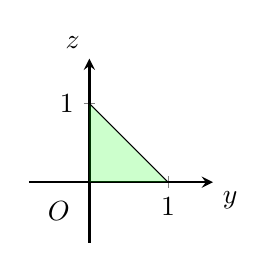
\begin{tikzpicture}
    \begin{axis}[standard,
            xtick={1},
            ytick={1},
            samples=1000,
            xlabel={$y$},
            ylabel={$z$},
          xmin=-.5,
          xmax=1.3,          
          ymin=-.5,
          ymax=1.3,
            x=1cm,
            y=1cm/1,
           ]

    \node[anchor=center,label=south west:$O$] at (axis cs:0,0){};
\addplot[name path=F,domain={0:1}]{1-x};
\addplot[name path=G,domain={0:1}]{0};
\addplot[fill=green, fill opacity=0.2] fill between [of=F and G, soft clip={domain=0:1}];
    \end{axis}
    \end{tikzpicture}
}
\end{center}

Our lower and upper bounds for $y$ are $y=0$ and $y=1$, respectively.

Our lower and upper bounds for $z$ are $z=0$ and $z=1-y$, respectively.

Since $g(x,y,z)=x$,
\begin{align*}
    \nabla g &=\lra{1,0,0}\\
    g_x&=1\\
    \frac{\norm{\nabla g}}{\left|g_x\right|}&=\frac{\sqrt{1^2+0^2+0^2}}{\left|1\right|}=\frac{\sqrt{1^2}}{1}=1
\end{align*}
Let's evaluate our integral.
\begin{align*}
    \iint_{S_3} y+z\,d\sigma &=\int_0^1\int_0^{1-y}\lrp{y+z}\lrp{1}\,dz\,dy\\
    &=\int_0^1\lrb{yz+\frac{1}{2}z^2}_0^{1-y}\,dy\\
    &=\int_0^1 y(1-y)+\frac{1}{2}(1-y)^2\,dy\\
    &=\int_0^1 y-y^2 +\frac{1}{2}\lrp{1-2y+y^2}\,dy\\
    &=\int_0^1 y-y^2+\frac{1}{2}-y+\frac{1}{2}y^2\,dy\\
    &=\int_0^1 -\frac{1}{2}y^2 +\frac{1}{2}\,dy\\
    &=\lrb{-\frac{1}{6}y^3+\frac{1}{2}y}_0^1\\
    &=-\frac{1}{6}(1)^3+\frac{1}{2}(1)\\
    &=\frac{1}{3}
\end{align*}

\phantomsection
\addcontentsline{toc}{subsubsection}{x=2 Face}\textbf{$x=2$ Face}

On the $x=2$ face, let $g(x,y,z)=x=2$ where $x$ is a function implicitly defined by $y$ and $z$. 

Our lower and upper bounds for $y$ and $z$ come from $y+z=1$. If we define $z$ as a function of $y$, we get $z=1-y$.

Graphically, this looks like
\begin{center}
\resizebox{5cm}{!}{
    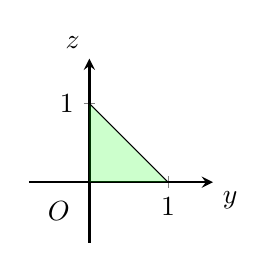
\begin{tikzpicture}
    \begin{axis}[standard,
            xtick={1},
            ytick={1},
            samples=1000,
            xlabel={$y$},
            ylabel={$z$},
          xmin=-.5,
          xmax=1.3,          
          ymin=-.5,
          ymax=1.3,
            x=1cm,
            y=1cm/1,
           ]

    \node[anchor=center,label=south west:$O$] at (axis cs:0,0){};
\addplot[name path=F,domain={0:1}]{1-x};
\addplot[name path=G,domain={0:1}]{0};
\addplot[fill=green, fill opacity=0.2] fill between [of=F and G, soft clip={domain=0:1}];
    \end{axis}
    \end{tikzpicture}
}
\end{center}

Our lower and upper bounds for $y$ are $y=0$ and $y=1$, respectively.

Our lower and upper bounds for $z$ are $z=0$ and $z=1-y$, respectively.

Since $g(x,y,z)=x=2$,
\begin{align*}
    \nabla g &=\lra{1,0,0}\\
    g_x&=1\\
    \frac{\norm{\nabla g}}{\left|g_x\right|}&=\frac{\sqrt{1^2+0^2+0^2}}{\left|1\right|}=\frac{\sqrt{1^2}}{1}=1
\end{align*}
Let's evaluate our integral.
\begin{align*}
      \iint_{S_4} y+z\,d\sigma&=\int_0^1\int_0^{1-y}\lrp{y+z}\lrp{1}\,dz\,dy\\
    &=\int_0^1\lrb{yz+\frac{1}{2}z^2}_0^{1-y}\,dy\\
    &=\int_0^1 y(1-y)+\frac{1}{2}(1-y)^2\,dy\\
    &=\int_0^1 y-y^2 +\frac{1}{2}\lrp{1-2y+y^2}\,dy\\
    &=\int_0^1 y-y^2+\frac{1}{2}-y+\frac{1}{2}y^2\,dy\\
    &=\int_0^1 -\frac{1}{2}y^2 +\frac{1}{2}\,dy\\
    &=\lrb{-\frac{1}{6}y^3+\frac{1}{2}y}_0^1\\
    &=-\frac{1}{6}(1)^3+\frac{1}{2}(1)\\
    &=\frac{1}{3}
\end{align*}

\phantomsection
\addcontentsline{toc}{subsubsection}{y+z=1 Face}\textbf{$y+z=1$ Face}

On the $y+z=1$ face, let $g(x,y,z)=y+z=1$ where $z$ be a function implicitly defined by $x$ and $y$. 

Our lower and upper bounds for $x$ are $x=0$ and $x=2$, respectively.

Our lower and upper bounds for $y$ are $y=0$ and $y+0=1\implies y=1$, respectively.

Since $g(x,y,z)=y+z$,
\begin{align*}
    \nabla g &= \lra{0,1,1}\\
    g_z &=1\\
    \frac{\norm{\nabla g}}{\left|g_z\right|}&=\frac{\sqrt{0^2+1^2+1^2}}{\left|1\right|}=\frac{\sqrt{1^2+1^2}}{1}=\sqrt{2}
\end{align*}
Let's evaluate our integral.
\begin{align*}
    \iint_{S_5} y+z\,d\sigma &=\int_0^2\int_0^1\lrp{y+z}\lrp{\sqrt{2}}\,dy\,dx\\
    &=\int_0^2\int_0^1\lrp{1}\lrp{\sqrt{2}}\,dy\,dx\tag{$y+z=1$}\\
    &=\int_0^2\int_0^1\sqrt{2}\,dy\,dx\\
    &=\int_0^2 \lrb{\sqrt{2}y}_0^1\,dx\\
    &=\int_0^2 \sqrt{2}\,dx\\
    &=\lrb{\sqrt{2}x}_0^2\\
    &=2\sqrt{2}
\end{align*}
Our final answer is
\begin{align*}
   \iint_S y+z\,d\sigma&=\iint_{S_1} y+z\,d\sigma+\iint_{S_2} y+z\,d\sigma+\iint_{S_3} y+z\,d\sigma+\iint_{S_4} y+z\,d\sigma+\iint_{S_5} y+z\,d\sigma\\ &=1+1+\frac{1}{3}+\frac{1}{3}+2\sqrt{2}\\
   &=\boxed{\frac{8}{3}+2\sqrt{2}}
\end{align*}

\phantomsection
\addcontentsline{toc}{subsection}{1(e)}\textbf{(e)} $f(x,y,z)=xyz$ over the surface of the rectangular solid cut from the first octant by the planes $x=a$, $y=b$, $z=c$

\Solution

A rectangular solid has $6$ faces, so we'll probably need to evaluate $6$ surface integrals right?

Nope. $3$ of these integrals will just evaluate to $0$. Please see today's lecture (5/16) for why.

Therefore, we only need to evaluate $3$ surfaces integrals: one for $x=a$, one for $y=b$, and one for $z=c$.

\phantomsection
\addcontentsline{toc}{subsubsection}{x=a Face}\textbf{$x=a$ Face}

On the $x=a$ face, let $g(x,y,z)=x=a$ where $x$ is a function implicitly defined by $y$ and $z$.

Our lower and upper bounds for $y$ are $y=0$ and $y=b$, respectively.

Our lower and upper bounds for $z$ are $z=0$ and $z=c$, respectively.

Since $g(x,y,z)=x$,
\begin{align*}
    \nabla g&=\lra{1,0,0}\\
    g_x&=1\\
    \frac{\norm{\nabla g}}{\left|g_x\right|}&=\frac{\sqrt{1^2+0^2+0^2}}{\left|1\right|}=\frac{\sqrt{1^2}}{1}=1
\end{align*}
Let's evaluate our integral.
\begin{align*}
   \iint_{S_1}xyz\,d\sigma &=\int_0^b\int_0^c \lrp{ayz}\lrp{1}\,dz\,dx\\
    &=\int_0^c \lrb{\frac{1}{2}ayz^2}_0^c\,dy\\
    &=\int_0^b \frac{1}{2}ac^2y\,dy\\
    &=\lrb{\frac{1}{4}ac^2y^2}_0^b\\
    &=\frac{1}{4}ab^2c^2
\end{align*}

\phantomsection
\addcontentsline{toc}{subsubsection}{y=b Face}\textbf{$y=b$ Face}

On the $y=b$ face, let $g(x,y,z)=y=b$ where $y$ is a function implicitly defined by $x$ and $z$. 

Our lower and upper bounds for $x$ are $x=0$ and $x=a$, respectively.

Our lower and upper bounds for $z$ are $z=0$ and $z=c$, respectively.

Since $g(x,y,z)=y$,
\begin{align*}
    \nabla g &=\lra{0,1,0}\\
    g_y&=1\\
    \frac{\norm{\nabla g}}{g_y}&=\frac{\sqrt{0^2+1^2+0^2}}{\left|1\right|}=\frac{\sqrt{1^2}}{1}=1
\end{align*}
Let's evaluate our integral.
\begin{align*}
  \iint_{S_2}xyz\,d\sigma   &=\int_0^a\int_0^c \lrp{xbz}\lrp{1}\,dz\,dx\\
    &=\int_0^a \lrb{\frac{1}{2}bxz^2}_0^c\,dx\\
    &=\int_0^a \frac{1}{2}bc^2 x\,dx\\
    &=\lrb{\frac{1}{4}bc^2x^2}_0^a\\
    &=\frac{1}{4}a^2bc^2
\end{align*}

\phantomsection
\addcontentsline{toc}{subsubsection}{z=c Face}\textbf{$z=c$ Face}

On the $z=c$ face, let $g(x,y,z)=z=c$ where $z$ is a function implicitly defined by $x$ and $y$.

Our lower and upper bounds for $x$ are $x=0$ and $x=a$, respectively.

Our lower and upper bounds for $z$ are $z=0$ and $z=c$, respectively.

Since $g(x,y,z)=z$,
\begin{align*}
    \nabla g &=\lra{0,0,1}\\
    g_z&=1\\
    \frac{\norm{\nabla g}}{g_z}&=\frac{\sqrt{0^2+0^2+1^2}}{\left|1\right|}=\frac{\sqrt{1^2}}{1}=1
\end{align*}
Let's evaluate the integral.
\begin{align*}
    \iint_{S_3}xyz\,d\sigma &=\int_0^a\int_0^b \lrp{xyc}\lrp{1}\,dy\,dx\\
    &=\int_0^a \lrb{\frac{1}{2}cxy^2}_0^b\,dx\\
    &=\int_0^a \frac{1}{2}b^2cx\,dx\\
    &=\lrb{\frac{1}{4}b^2cx^2}_0^a\\
    &=\frac{1}{4}a^2b^2c
\end{align*}
Our final answer is
\begin{align*}
    \frac{1}{4}ab^2c^2+\frac{1}{4}a^2bc^2+\frac{1}{4}a^2b^2c=\frac{ab^2c^2+a^2bc^2+a^2b^2c}{4}=\frac{abc(bc+ac+ab)}{4}=\boxed{\frac{abc(ab+ac+bc)}{4}}
\end{align*}

\phantomsection
\addcontentsline{toc}{subsection}{1(f)}\textbf{(f)} $f(x,y,z)=x+y+z$ over the portion of the plane $2x+2y+z=2$ that lies in the first octant

\Solution

Let $g(x,y,z)=2x+2y+z$ where $z$ is implicitly defined by $x$ and $y$. 

We can get our lower and upper bounds for $x$ and $y$ from the shadow in the $xy$-plane ($z=0$).

When $z=0$, $2x+2y+0=2\implies 2x+2y=2\implies x+y=1\implies y=1-x$.

Graphically, this looks like
\begin{center}
\resizebox{5cm}{!}{
    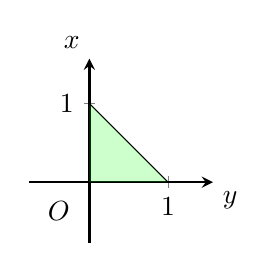
\begin{tikzpicture}
    \begin{axis}[standard,
            xtick={1},
            ytick={1},
            samples=1000,
            xlabel={$y$},
            ylabel={$x$},
          xmin=-.5,
          xmax=1.3,          
          ymin=-.5,
          ymax=1.3,
            x=1cm,
            y=1cm/1,
           ]

    \node[anchor=center,label=south west:$O$] at (axis cs:0,0){};
\addplot[name path=F,domain={0:1}]{1-x};
\addplot[name path=G,domain={0:1}]{0};
\addplot[fill=green, fill opacity=0.2] fill between [of=F and G, soft clip={domain=0:1}];
    \end{axis}
    \end{tikzpicture}
}
\end{center}

Our lower and upper bounds for $x$ are $x=0$ and $x=1$, respectively.

Our lower and upper bounds for $y$ are $y=0$ and $y=1-x$, respectively.

Since $g(x,y,z)=2x+2y+z$,
\begin{align*}
    \nabla g&=\lra{2,2,1}\\
    g_z&=1\\
    \frac{\norm{\nabla g}}{\left|g_z\right|}&=\frac{\sqrt{2^2+2^2+1^2}}{\left|1\right|}=\frac{\sqrt{9}}{1}=3
\end{align*}
Let's evaluate the integral.
\begin{align*}
     \iint_{S}x+y+z\,d\sigma&=\int_0^1\int_0^{1-x}\big(x+y+\lrp{2-2x-2y}\big)\lrp{3}\,dy\,dx\tag{$2x+2y+z=2\implies z=2-2x-2y$}\\
    &=\int_0^1\int_0^{1-x}\lrp{-x-y+2}\lrp{3}\,dy\,dx\\
    &=\int_0^1 \int_0^{1-x}-3x-3y+6\,dy\,dx\\
    &=\int_0^1 \lrb{-3xy-\frac{3}{2}y^2+6y}_0^{1-x}\,dx\\
    &=\int_0^1 -3x(1-x)-\frac{3}{2}(1-x)^2+6(1-x)\,dx\\
    &=\int_0^1 -3x+3x^2-\frac{3}{2}(1-2x+x^2)+6-6x\,dx\\
    &=\int_0^1-3x+3x^2-\frac{3}{2}+3x-\frac{3}{2}x^2+6-6x\,dx\\
    &=\int_0^1 \frac{3}{2}x^2 -6x +\frac{9}{2}\,dx\\
    &=\lrb{\frac{1}{2}x^3-3x^2+\frac{9}{2}x}_0^1\\
    &=\frac{1}{2}(1)^3-3(1)^2+\frac{9}{2}(1)\\
    &=\boxed{2}\tag{use a calculator}
\end{align*}
\phantomsection
\addcontentsline{toc}{subsection}{1(g)}\textbf{(g)} $f(x,y,z)=x\sqrt{y^2+4}$ over the surface cut from the parabolic cylinder $y^2+4z=16$ by the planes $x=0$, $x=1$, and $z=0$

\Solution

Let $g(x,y,z)=y^2+4z$ where $z$ is implicitly defined by $x$ and $y$. 

Our lower and upper bounds for $x$ are $x=0$ and $x=1$, respectively.

We can get our lower and upper bounds for $y$ from $z=0$. If $z=0$, then $y^2+4(0)=16\implies y^2=16\implies y=\pm 4$.

Our lower and upper bonds for $y$ are $y=-4$ and $y=4$, respectively.

Since $g(x,y,z)=y^2+4z$,
\begin{align*}
    \nabla g &=\lra{0,2y,4}\\
    g_z&=4\\
    \frac{\norm{\nabla g}}{\left|g_z\right|}&=\frac{\sqrt{0+(2y)^2+4^2}}{\left|4\right|}=\frac{4y^2+16}{4}=\frac{\sqrt{4}\sqrt{y^2+4}}{4}=\frac{\sqrt{y^2+4}}{2}\tag{$\sqrt{4}=2$}
\end{align*}
Let's evaluate the integral.
\begin{align*}
    \iint_{S}x\sqrt{y^2+4}\,d\sigma &=\int_0^1 \int_{-4}^4 \lrp{x\sqrt{y^2+4}}\lrp{\frac{\sqrt{y^2+4}}{2}}\,dy\,dx\\
    &=\int_0^1 \int_{-4}^4 \frac{x}{2}\lrp{y^2+4}\,dy\,dx\\
    &=\int_{-4}^4\int_0^1 \frac{x}{2}\lrp{y^2+4}\,dx\,dy\tag{the other order looked dreadful}\\
    &=\int_{-4}^4 \lrb{\frac{x^2}{4}(y^2+4)}_0^1\,dy\\
    &=\int_{-4}^4 \frac{1^2}{4}\lrp{y^2+4}\,dy\\
    &=\int_{-4}^4 \frac{1}{4}y^2+1\,dy\\
    &=\lrb{\frac{1}{12}y^3+y}_{-4}^4\\
    &=\lrp{\frac{1}{12}(4)^3+4}-\lrp{\frac{1}{12}(-4)^3+(-4)}\\
    &=\lrp{\frac{28}{3}}-\lrp{-\frac{28}{3}}\tag{use a calculator}\\
    &=\boxed{\frac{56}{3}}
\end{align*}

\phantomsection
\addcontentsline{toc}{subsection}{1(h)}\textbf{(h)} $f(x,y,z)=z-x$ over the portion of the graph of $z=x+y^2$ above the triangle in the $xy$-plane with vertices $(0,0,0)$, $(1,1,0)$ and $(0,1,0)$

\Solution

Let $g(x,y,z)=-x-y^2+z$ where $z$ is implicitly defined by $x$ and $y$. 

We can get our lower and upper bounds for $x$ and $y$ from the triangle $(0,0)$, $(1,1)$, and $(0,1)$.


Graphically, this looks like
\begin{center}
\resizebox{3.5cm}{!}{
    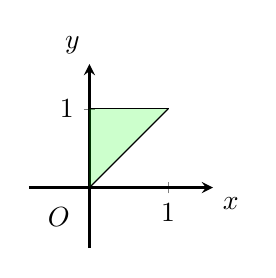
\begin{tikzpicture}
    \begin{axis}[standard,
            xtick={1},
            ytick={1},
            samples=1000,
            xlabel={$x$},
            ylabel={$y$},
          xmin=-.5,
          xmax=1.3,          
          ymin=-.5,
          ymax=1.3,
            x=1cm,
            y=1cm/1,
           ]

    \node[anchor=center,label=south west:$O$] at (axis cs:0,0){};
\addplot[name path=F,domain={0:1}]{x};
\addplot[name path=G,domain={0:1}]{1};
\addplot[fill=green, fill opacity=0.2] fill between [of=F and G, soft clip={domain=0:1}];
    \end{axis}
    \end{tikzpicture}
}
\end{center}

Looks like we have the line $y=x$ (find a line between $(0,0)$ and $(1,1)$) and $y=0$.

Our lower and upper bounds for $x$ are $x=0$ and $x=y$, respectively.

Our lower and upper bounds for $y$ are $y=0$ and $y=1$, respectively.

Trust me when I say we want to do $dx\,dy$ order instead of the regular $dy\,dx$ order.

... or don't and try doing the dreadful integral yourself D:

Since $g(x,y,z)=x-y^2+z$,
\begin{align*}
    \nabla g&=\lra{-1,-2y,1}\\
    g_z&=1\\
    \frac{\norm{\nabla g}}{\left|g_z\right|}&=\frac{\sqrt{(-1)^2+(-2y)^2+1^2}}{\left|1\right|}=\sqrt{1+4y^2+1}=\sqrt{4y^2+2}=\sqrt{2}\sqrt{2y^2+1}
\end{align*}
Let's evaluate the integral.
\begin{align*}
    \iint_{S}z-x\,d\sigma &=\int_0^1\int_0^y \lrp{\lrp{x+y^2}-x}\lrp{\sqrt{2}\sqrt{2y^2+1}}\,dx\,dy\\
    &=\int_0^1\int_0^y\lrp{y^2}\lrp{\sqrt{2}\sqrt{2y^2+1}}\,dx\,dy\\
    &=\int_0^1 \lrb{\lrp{xy^2}\lrp{\sqrt{2}\sqrt{2y^2+1}}}_0^y\,dy\\
    &=\int_0^1 \lrp{y^3}\lrp{\sqrt{2}\sqrt{2y^2+1}}\,dy\\
    &=\sqrt{2}\int_0^1 y^3\sqrt{2y^2+1}\tag{we can take constants out}\\
    &u=2y^2+1; \frac{u-1}{2}=y^2\hspace{2em}du=4y\,dy\\
    &u(0)=1\hspace{2em}u(1)=3\\
    &=\frac{\sqrt{2}}{4}\int_1^3 \lrp{\frac{u-1}{2}}\sqrt{u}\,du\\
    &=\frac{\sqrt{2}}{4}\int_1^3 \frac{1}{2}u^{3/2}-\frac{1}{2}u^{1/2}\,du\\
    &=\frac{\sqrt{2}}{4}\lrb{\frac{1}{5}u^{5/2}-\frac{1}{3}u^{3/2}}_1^3\\
    &=\frac{\sqrt{2}}{4}\Bigg(\lrp{\frac{1}{5}(3)^{5/2}-\frac{1}{3}(3)^{3/2}}-\lrp{\frac{1}{5}-\frac{1}{3}}\Bigg)\\
    &=\frac{\sqrt{2}}{4}\Bigg(\lrp{\frac{1}{5}(9)(\sqrt{3})-\frac{1}{3}(3)(\sqrt{3})}-\lrp{-\frac{2}{15}}\Bigg)\\
    &=\frac{\sqrt{2}}{4}\Bigg(\lrp{\frac{27\sqrt{3}}{15}-\frac{15\sqrt{3}}{15}}+\frac{2}{15}\Bigg)\\
    &=\frac{\sqrt{2}}{4}\Bigg(\frac{12\sqrt{3}}{15}+\frac{2}{15}\Bigg)\\
    &=\frac{12\sqrt{6}}{60}+\frac{2\sqrt{2}}{60}\\
    &=\frac{6\sqrt{6}}{30}+\frac{\sqrt{2}}{30}\\
    &=\boxed{\frac{6\sqrt{6}+\sqrt{2}}{30}}
\end{align*}
\phantomsection
\addcontentsline{toc}{section}{Problem 2 (Parts)}\textbf{Problem 2 (Parts)}

On Homework 11, we used a line integral to calculate the mass and center of mass
of a wire in space. We can similarly use a surface integral to calculate the mass and
center of mass of a shell whose density at $(x,y,z)$ is $\delta(x,y,z)$. The mass is given by
\begin{equation*}
    M=\iint_S \delta (x,y,z)\,d\sigma
\end{equation*}
and we can also write integral formulas for the moments around the coordinate planes.

\phantomsection
\addcontentsline{toc}{subsection}{(a)}\textbf{(a)} Find the centroid of the portion of the sphere $x^2+y^2+z^2=a^2$ in the first octant.

\Solution

Let's \textit{not} use a surface integral (directly) to calculate the mass of a shell. Instead, let's use the surface area of a sphere formula.
\begin{align*}
    M=\iint_S \delta(x,y,z)\,d\sigma &=\delta(x,y,z)\lrp{\text{surface area of first octant}}=\delta(x,y,z)\lrp{\frac{1}{8}(4\pi a^2)}=\frac{1}{2}\delta(x,y,z)\pi a^2
\end{align*}
By symmetry, $\overline{x}=\overline{y}=\overline{z}$ since a sphere in the first octant is symmetrical.

Let's just find what $M_{xy}$ is to find what $\overline{z}$ is.

Let $g(x,y,z)=x^2+y^2+z^2$ where $z$ is implicitly defined by $x$ and $y$. Then,
\begin{align*}
    \nabla g&=\lra{2x,2y,2z}\\
    g_z&=2z\\
    \frac{\norm{\nabla g}}{\left|g_z\right|}&=\frac{\sqrt{(2x)^2+(2y)^2+(2z)^2}}{\left|2z\right|}=\frac{\sqrt{4x^2+4y^2+4z^2}}{2z}=\frac{\sqrt{4(x^2+y^2+z^2)}}{2z}=\frac{\sqrt{4(a^2)}}{2z}=\frac{2a}{2z}=\frac{a}{z}
\end{align*}
It sounds kind of awful to do this without cylindrical coordinates, so let's convert our region.

Our region is the shadow in the $xy$ plane ($z=0$) which is just $x^2+y^2+0^2=a^2\implies x^2+y^2=a^2$ ($x,y\geq 0$). Our region is a quarter with radius $a$ in the first quadrant (since we're in the first octant). Therefore, our lower and upper bounds for $r$ are $r=0$ and $r=a$, respectively.

Our lower and upper bounds for $\theta$ are $\theta=0$ and $\theta=\dfrac{\pi}{2}$, respectively.

Let's find $M_{xy}$.
\begin{align*}
    M_{xy}&=\int_0^{\pi/2}\int_0^a z\delta(x,y,z)\lrp{\frac{a}{z}}\lrp{r}\,dr\,d\theta\\
    &=\int_0^{\pi/2}\int_0^a \delta(x,y,z)ar\,dr\,d\theta\\
    &=\int_0^{\pi/2}\lrb{\frac{1}{2}\delta(x,y,z)ar^2}_0^a\,d\theta\\
    &=\int_0^{\pi/2}\frac{1}{2}\delta(x,y,z)a^3\,d\theta\\
    &=\lrb{\frac{1}{2}\delta(x,y,z)a^3\theta}_0^{\pi/2}\\
    &=\frac{1}{2}\delta(x,y,z)a^3\lrp{\frac{\pi}{2}}\\
    &=\frac{1}{4}\delta(x,y,z)\pi a^3
\end{align*}
Since $\displaystyle M=\frac{1}{2}\delta(x,y,z)\pi a^2$ and $\displaystyle M_{xy}=\frac{1}{4}\delta(x,y,z)\pi a^3$,
\begin{align*}
    \overline{z}&=\frac{\frac{1}{4}\delta(x,y,z)\pi a^3}{\frac{1}{2}\delta(x,y,z)\pi a^2}=\frac{1}{2}a
\end{align*}
Since $\overline{x}=\overline{y}=\overline{z}$, the centroid is
\begin{equation*}
    \boxed{\lrp{\frac{1}{2}a,\frac{1}{2}a,\frac{1}{2}a}}
\end{equation*}

\phantomsection
\addcontentsline{toc}{subsection}{(b)}\textbf{(b)} A surface $S$ lies on the paraboloid $z=\frac{1}{2}x^2+\frac{1}{2}y^2$ directly above the triangle in the $xy$-plane with vertices $(0,0)$, $(2,0)$ and $(2,4)$. If the density at a point $(x,y,z)$ on $S$ is given by $\delta(x,y,z)=9xy$, find the mass of $S$.

\Solution

Let $g(x,y,z)=-\frac{1}{2}x^2-\frac{1}{2}y^2+z$ where $z$ is implicitly defined by $x$ and $y$. Then,
\begin{align*}
    \nabla g&=\lra{-x,-y,1}\\
    g_z&=1\\
    \frac{\norm{\nabla g}}{\left|g_z\right|}&=\frac{\sqrt{(-x)^2+(-y)^2+1^2}}{\left|1\right|}={\sqrt{x^2+y^2+1}}
\end{align*}
We can find our lower and upper bounds for $x$ and $y$ from the triangle $(0,0)$, $(2,0)$ and $(2,4)$.

Graphically, this looks like
\begin{center}
\resizebox{3cm}{!}{
    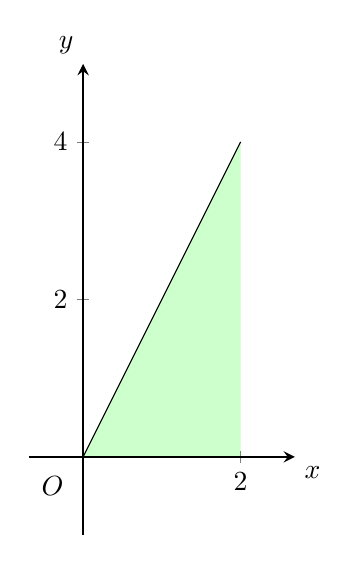
\begin{tikzpicture}
    \begin{axis}[standard,
            xtick={2},
            ytick={2,4},
            samples=1000,
            xlabel={$x$},
            ylabel={$y$},
            xmin=-0.3,xmax=2.3,
            ymin=-0.3,ymax=4.3,
            x=1cm,
            y=1cm/1,
           ]
\node[anchor=center,label=south west:$O$] at (axis cs:0,0){};
\addplot[name path=F,domain={0:2}]{2*x};
\addplot[name path=G,domain={0:2}]{0};
\addplot[fill=green, fill opacity=0.2] fill between [of=F and G, soft clip={domain=0:2}];
    \end{axis}
    \end{tikzpicture}
}
\end{center}
Our lower and upper bounds for $y$ are $y=0$ and $y=2x$, respectively.

Our lower and upper bounds for $x$ are $x=0$ and $=2$, respectively.

Let's evaluate the integral.
\begin{align*}
    M&=\iint_S \delta(x,y,z)\,d\sigma\\
    &=\int_0^2\int_0^{2x}\lrp{9xy}\lrp{\sqrt{x^2+y^2+1}}\,dy\,dx\\
    &u=x^2+y^2+1\hspace{2em}du=2y\,dy\\
    &u(0)=x^2+1\hspace{2em}u(2x)=x^2+(2x)^2+1=5x^2+1\\
    &=\int_0^2 \int_{x^2+1}^{5x^2+1}\frac{9}{2}x\sqrt{u}\,du\,dx\\
    &=\int_0^2 \lrb{3xu^{3/2}}_{x^2+1}^{5x^2+1}\,dx\\
    &=\int_0^2 3x\lrp{5x^2+1}^{3/2}-3x\lrp{x^2+1}^{3/2}\,dx\\
    &=\underbrace{\int_0^2 3x(5x^2+1)^{3/2}\,dx}_{t-sub}-\underbrace{\int_0^2 3x(x^2+1)^{3/2}\,dx}_{v-sub}\\
    &t=5x^2+1\hspace{2em}dt=10x\,dx\\
    &t(0)=1\hspace{2em}t(2)=5(2)^2+1=21\\
    &v=x^2+1\hspace{2em}dv=2x\,dx\\
    &v(0)=1\hspace{2em}v(2)=(2)^2+1=5\\
    &=\int_1^{21}\frac{3}{10}t^{3/2}\,dt-\int_1^5 \frac{3}{2}v^{3/2}\,dv\\
    &=\lrb{\frac{3}{25}t^{5/2}}_1^{21}-\lrb{\frac{3}{5}v^{5/2}}_1^5\\
    &=\lrp{\frac{3}{25}(21)^{5/2}-\frac{3}{25}}-\lrp{\frac{3}{5}(5)^{5/2}-\frac{3}{5}}\\
    &=\frac{3}{25}(21)^{5/2}-\frac{3}{25}-\lrp{3(5)^{3/2}-\frac{3}{5}}\\
    &=\frac{3}{25}-\frac{3}{25}-3(5)^{3/2}+\frac{3}{5}\\
    &=\boxed{\frac{3}{25}(21)^{5/2}-3(5)^{3/2}+\frac{12}{15}}
\end{align*}
\end{document}
